\documentclass{article}
\usepackage{tikz}
\usepackage{pgf-pie}
\usepackage{pgf-umlsd}
\begin{document}
\emph{\subsection{Netflix Time Distribution}}
\begin{center}
\textbf{ NETFLIX}
\end{center}

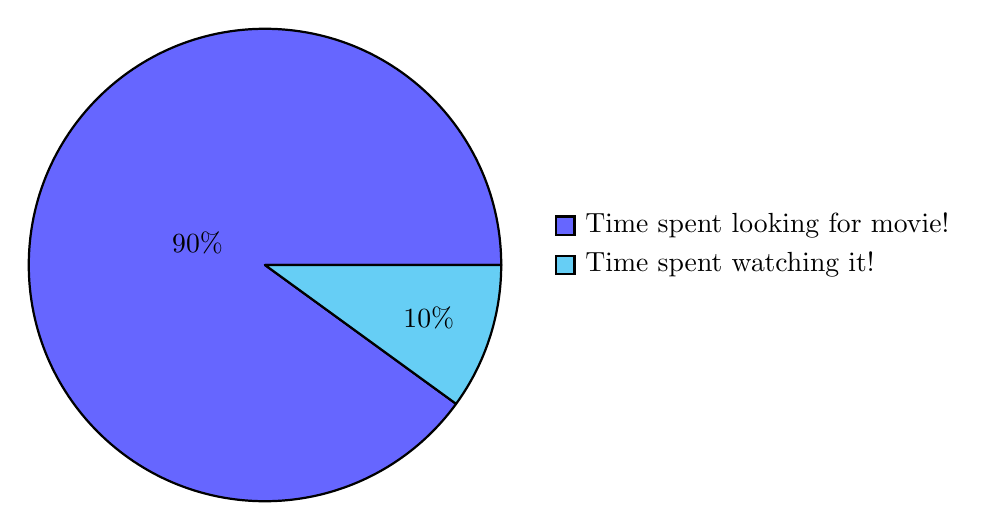
\begin{tikzpicture}
    \pie[text=legend, radius=3]{
        90/Time spent looking for movie!,
        10/Time spent watching it!}
\end{tikzpicture}
\emph{\subsection{Daily Activities}}
\begin{center}
\textbf{ "Daily Activities"}
\end{center}

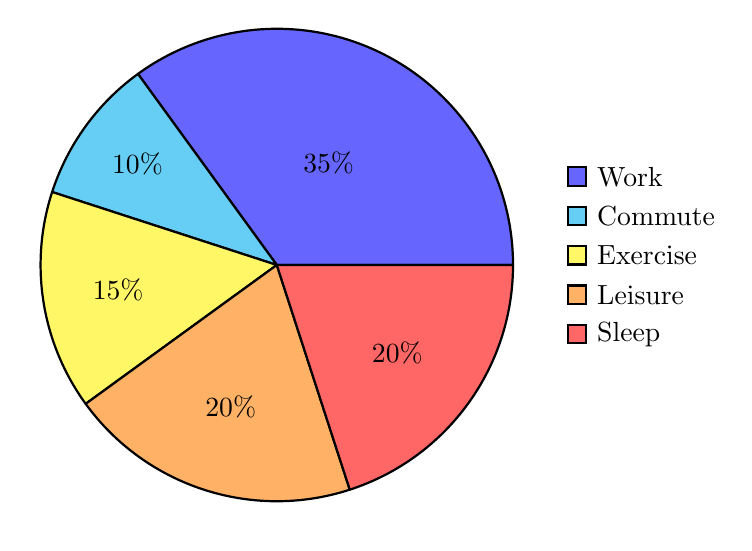
\begin{tikzpicture}
    \pie[text=legend, radius=3]{
        35/Work,
        10/Commute,
        15/Exercise,
        20/Leisure,
        20/Sleep}
\end{tikzpicture}
\emph{\subsection{Project Task Breakdown}}
\begin{center}
\textbf{ "Project Task Breakdown"}
\end{center}

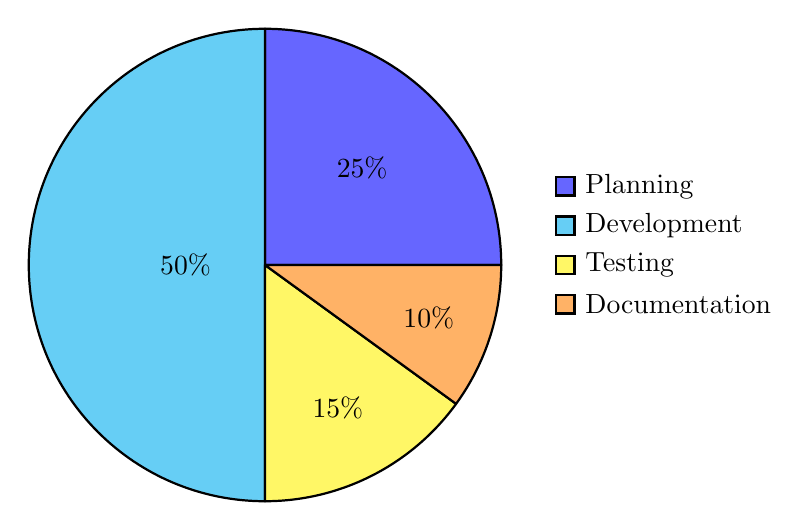
\begin{tikzpicture}
    \pie[text=legend, radius=3]{
        25/Planning,
        50/Development,
        15/Testing,
        10/Documentation}
\end{tikzpicture}
\emph{\subsection{Browser Market Share}}
\begin{center}
\textbf{ "Browser Market Share 2024"}
\end{center}

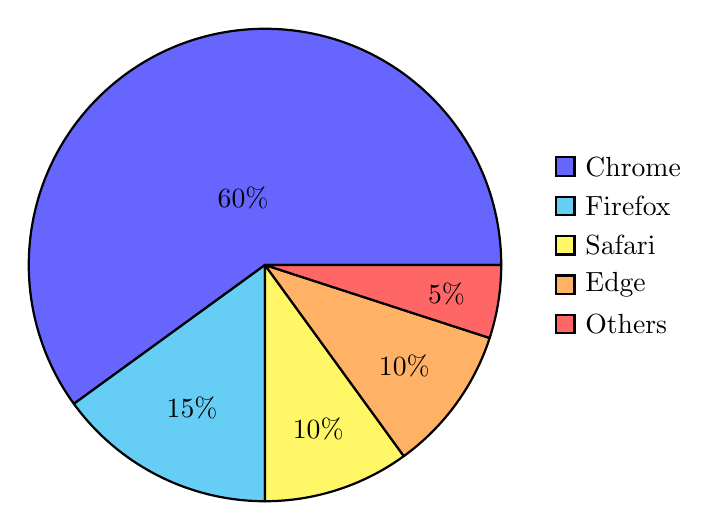
\begin{tikzpicture}
    \pie[text=legend, radius=3]{
        60/Chrome,
        15/Firefox,
        10/Safari,
        10/Edge,
        5/Others}
\end{tikzpicture}
\emph{\subsection{Favorite Food}}
\begin{center}
\textbf{ "Favorite Food Poll"}
\end{center}

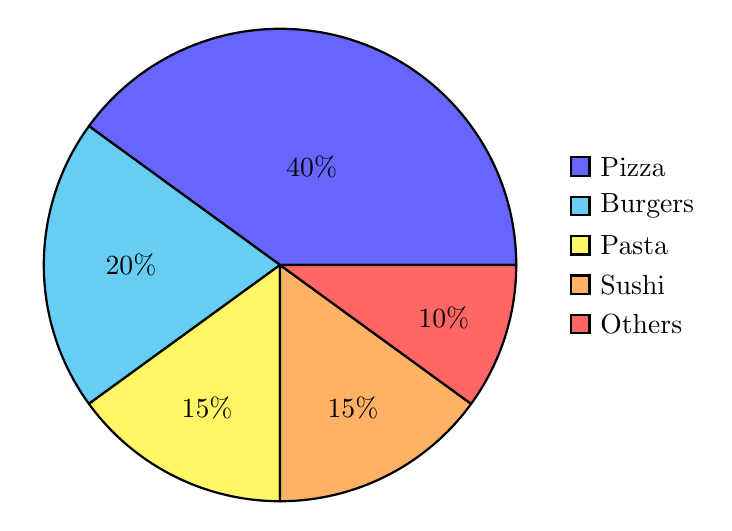
\begin{tikzpicture}
    \pie[text=legend, radius=3]{
        40/Pizza,
        20/Burgers,
        15/Pasta,
        15/Sushi,
        10/Others}
\end{tikzpicture}
\end{document}
